 \documentclass{beamer}[10]

\usepackage{graphicx}
\usepackage{xcolor}
\usepackage{tabto}
%\usepackage{beamerthemesplit}
\usepackage{tikz}
\usepackage{cancel}
\usepackage{verbatim}
\usepackage{fancybox}
\usepackage{enumerate}
\usepackage{amsmath,amssymb,amsthm,textcomp,mathtools}
\usepackage[super]{nth}
\usepackage[amssymb]{SIunits}
\usepackage{booktabs}
\usepackage{cancel}
\usepackage{bm}
\usepackage[utf8]{inputenc}
\usepackage{tabularx}
\usepackage{ragged2e}
\newcolumntype{Y}{ >{\RaggedRight\arraybackslash}X}
\usetikzlibrary{arrows,shapes}
\newcommand\T{\rule{0pt}{2.6ex}}
\newcommand\B{\rule[-1.2ex]{0pt}{0pt}}
\definecolor{UUcrimson}{RGB}{204,0,0}
\mode<presentation>
{ \usetheme{default}
  \usecolortheme[named=UUcrimson]{structure}
  \useinnertheme{circles}
  \setbeamercovered{transparent}
  \setbeamertemplate{blocks}[rounded]
  \usefonttheme[onlymath]{serif}
  \setbeamertemplate{navigation symbols}{}
  \setbeamertemplate{footline}[page number]
  \setbeamertemplate{navigation symbols}{}
  \setbeamercolor{section in toc}{fg=black,bg=white}
  \setbeamercolor{alerted text}{fg=UUcrimson!80!gray}
  \setbeamercolor*{palette primary}{fg=white,bg=UUcrimson}
  \setbeamercolor*{palette secondary}{fg=UUcrimson!70!black,bg=gray!15!white}
  \setbeamercolor*{palette tertiary}{bg=UUcrimson!80!black,fg=gray!10!white}
  \setbeamercolor*{palette quaternary}{fg=UUcrimson,bg=gray!5!white}
  \setbeamercolor*{palette sidebar primary}{fg=UUcrimson!10!black}
  \setbeamercolor*{palette sidebar secondary}{fg=white}
  \setbeamercolor*{palette sidebar tertiary}{fg=UUcrimson!50!black}
  \setbeamercolor*{palette sidebar quaternary}{fg=gray!10!white}
  \setbeamercolor{titlelike}{parent=palette primary,fg=white}
  \setbeamercolor{frametitle}{bg=UUcrimson}
  \setbeamercolor{frametitle right}{bg=UUcrimson}
  \setbeamercolor*{separation line}{}
  \setbeamercolor*{fine separation line}{}
}

\usetikzlibrary{backgrounds}
\makeatletter
\tikzstyle{every picture}+=[remember picture]
\tikzset{%
  fancy quotes/.style={
    text width=\fq@width pt,
    align=justify,
    inner sep=1em,
    anchor=north west,
    minimum width=\linewidth,
    font=\itshape
  },
  fancy quotes width/.initial={.8\linewidth},
  fancy quotes marks/.style={
    scale=8,
    text=white,
    inner sep=0pt,
  },
  fancy quotes opening/.style={
    fancy quotes marks,
  },
  fancy quotes closing/.style={
    fancy quotes marks,
  },
  fancy quotes background/.style={
    show background rectangle,
    inner frame xsep=0pt,
    background rectangle/.style={
      fill=gray!25,
      rounded corners,
    },
  }
}
\newenvironment{fancyquotes}[1][]{%
\noindent
\tikzpicture[fancy quotes background]
\node[fancy quotes opening,anchor=north west] (fq@ul) at (0,0) {``};
\tikz@scan@one@point\pgfutil@firstofone(fq@ul.east)
\pgfmathsetmacro{\fq@width}{\linewidth - 2*\pgf@x}
\node[fancy quotes,#1] (fq@txt) at (fq@ul.north west) \bgroup}
{\egroup;
\node[overlay,fancy quotes closing,anchor=east] at (fq@txt.south east) {''};
\endtikzpicture}
\makeatother

\usepackage{scalerel}[2014/03/10]
\usepackage{stackengine}
\usepackage{empheq}
\newcommand*\widefbox[1]{\fbox{\hspace{0.5em}#1\hspace{0.5em}}}

\newcommand\reallywidetilde[1]{\ThisStyle{%
  \setbox0=\hbox{$\SavedStyle#1$}%
  \stackengine{-.1\LMpt}{$\SavedStyle#1$}{%
    \stretchto{\scaleto{\SavedStyle\mkern.2mu\sim}{.5467\wd0}}{.4\ht0}%
%    .2mu is the kern imbalance when clipping white space
%    .5467++++ is \ht/[kerned \wd] aspect ratio for \sim glyph
  }{O}{c}{F}{T}{S}%
}}
\usepackage{media9}

\logo{
\includegraphics[width=0.75cm]{logo.jpg}}
\author[Gibbs]{Dr. Jeremy A. Gibbs}
\institute{Department of Mechanical Engineering\\University of Utah}
\date{Fall 2016}
\title{LES of Turbulent Flows: Lecture 15}
\begin{document}

%----------------------------------------------------------------------------------------
%	TITLE & TOC SLIDES
%----------------------------------------------------------------------------------------

\begin{frame} 
  \titlepage
\end{frame}

%------------------------------------------------

\begin{frame}
\frametitle{Overview}
\tableofcontents
\end{frame}

%------------------------------------------------
\section{Similarity Models} %
%------------------------------------------------
\begin{frame}{Similarity Models}
\begin{itemize}
	\item So far we have focused on eddy-viscosity models and now we will look at similarity models (See Saguat pg 231 for examples)
	\item Scale similarity assumes that the statistical structure of tensors constructed on the basis of the SFS is similar to that of their equivalents evaluated on the basis of the smallest resolved scales
	\item Accordingly, the spectrum is usually separated into three bands
	\begin{itemize}
		\item the largest resolved scales
		\item the smallest resolved scales (also called the test field)
		\item the unresolved scales
	\end{itemize}
\end{itemize}

\end{frame}

%------------------------------------------------
\begin{frame}{Similarity Models}
\begin{itemize}
	\item The notion of scale similarity models can be interpreted in two ways
	\item One relates to energy cascade, with the idea that the unresolved scales and smallest resolved scales have a common history through interactions with largest scales
	\item The other relates to coherent structures, where some structures appear in each of the three bands and cause a strong correlation of the field among each level of decomposition
\end{itemize}

\end{frame}

%------------------------------------------------
\begin{frame}{Similarity Models}
\begin{itemize}
	\item Bardina et al., (1980) proposed an alternative model to the eddy-viscosity model
	\item They authors were motivated by the low correlations between $\tau_{ij}^{\Delta}(\vec{x},t)$ and $\tau_{ij}^{\Delta,M}(\vec{x},t)$ in \textit{a priori} studies
	\item We will cover \textit{a priori} studies in a later lecture
	\item The subgrid stress tensor is found by applying the filter a second time, which is a means to evaluate the fluctuation of the resolved scales
	\item As a result, this model cannot be used when the filter is idempotent because the fluctuation is zero
\end{itemize}

\end{frame}


%------------------------------------------------

\begin{frame}{Similarity Models}
\begin{itemize}
	\item Recall that the SFS velocity is defined as $u_i^\prime = u_i - \widetilde{u}_i$ and the filtered SFS velocity is $\widetilde{u_i^\prime} = \widetilde{u}_i - \widetilde{\widetilde{u}}_i$
	\item Also recall Leonard's decomposition of $\tau_{ij}$
	$$\tau_{ij} = L_{ij} + C_{ij} + R_{ij}$$
	where
	\begin{align*}
	L_{ij} &= \underbrace{\left(\widetilde{\widetilde{u}_i\widetilde{u}_j} - \widetilde{u}_i \widetilde{u}_j\right)	}_{\text{Resolved stresses}}\\\\
	C_{ij} &= \underbrace{\left(\widetilde{\widetilde{u}_i u_j^\prime} +\widetilde{u_i^\prime \widetilde{u}_j}\right)}_{\text{Cross stresses}}\\\\
	R_{ij} &= \underbrace{\widetilde{u_i^\prime u_j^\prime}}_{\text{``Reynolds'' stresses}}
	\end{align*}

\end{itemize}

\end{frame}

%------------------------------------------------

\begin{frame}{Similarity Models}
\begin{itemize}
	\item Using our definition of the filtered velocity fluctuations, and the following  assumption shown for $R_{ij}$, we can write each of our terms as follows
	\begin{align*}
	R_{ij} &= \reallywidetilde{\left(u_i - \widetilde{u}_i\right)\left(u_j - \widetilde{u}_j\right)}\\&\approx \left(\widetilde{u}_i - \widetilde{\widetilde{u}}_i\right)\left(\widetilde{u}_j - \widetilde{\widetilde{u}}_j\right)\\
	C_{ij} &\approx \widetilde{\widetilde{u}}_i\left(\widetilde{u}_j - \widetilde{\widetilde{u}}_j\right) + \widetilde{\widetilde{u}}_j\left(\widetilde{u}_i - \widetilde{\widetilde{u}}_i\right)\\
	L_{ij} &= \left(\widetilde{\widetilde{u}_i\widetilde{u}_j} - \widetilde{u}_i \widetilde{u}_j\right)
	\end{align*}

\end{itemize}

\end{frame}

%------------------------------------------------

\begin{frame}{Similarity Models}
\begin{itemize}
	\item Let's add them up and do a little algebra
	\begin{align*}
	\tau_{ij} = &\left(\widetilde{\widetilde{u}_i\widetilde{u}_j} - \widetilde{u}_i \widetilde{u}_j\right) + \widetilde{\widetilde{u}}_i\left(\widetilde{u}_j - \widetilde{\widetilde{u}}_j\right) + \widetilde{\widetilde{u}}_j\left(\widetilde{u}_i - \widetilde{\widetilde{u}}_i\right) \\&+\left(\widetilde{u}_i - \widetilde{\widetilde{u}}_i\right)\left(\widetilde{u}_j - \widetilde{\widetilde{u}}_j\right)\\
	= & \widetilde{u}_i \widetilde{u}_j - \widetilde{u}_i\widetilde{\widetilde{u}}_j  - \widetilde{\widetilde{u}}_i \widetilde{u}_j + \widetilde{\widetilde{u}}_i \widetilde{\widetilde{u}}_j + \widetilde{\widetilde{u}}_i\widetilde{u}_j - \widetilde{\widetilde{u}}_i \widetilde{\widetilde{u}}_j + \widetilde{\widetilde{u}}_j \widetilde{u}_i\\
	&- \widetilde{\widetilde{u}}_j\widetilde{\widetilde{u}}_i + \left(\widetilde{\widetilde{u}_i\widetilde{u}_j} - \widetilde{u}_i \widetilde{u}_j\right)
	\end{align*}
	Simple elimination yields
	$$\boxed{\tau_{ij} = \left(\widetilde{\widetilde{u}_i\widetilde{u}_j} - \widetilde{\widetilde{u}}_i\widetilde{\widetilde{u}}_j\right)}$$
	which gives an estimate for the SGS stress
\end{itemize}

\end{frame}

%------------------------------------------------

\begin{frame}{Similarity Models}
\begin{itemize}
	\item The Bardina model does not require physical modeling of SFSs, rather it is a mathematical approximation of $\tau_{ij}$
	\item \textit{a priori} tests against DNS databases showed that the Bardina model performed well
	\item The model produced high correlations with the true subgrid stress tensor
	\item These correlations occurred for both isotropic and anisotropic flows
	\item However, results also showed that the model is only slightly dissipative and underestimates the energy cascade
	\item The model also has a built in backscatter mechanism
\end{itemize}

\end{frame}

%------------------------------------------------

\begin{frame}{Similarity Models}
\begin{itemize}
	\item The Bardina model applied the same filter twice, meaning it used a single cutoff scale
	\item Liu et al. (1994) generalized the Bardina model to allow the use of filters with different shapes and widths, which allows it to be used for any type of filter.
	\item The authors examined ``bands'' around $\Delta$ and built a scale-similarity model similar to the model of Bardina et al. (1980)
	\item They argued that energy in the band at one scale larger than $\Delta$ (say $2\Delta$) and one scale  smaller (something like $0.5\Delta$) would have the largest contribution to $\tau_{ij}$.
\end{itemize}
\end{frame}

%------------------------------------------------

\begin{frame}{Similarity Models}
\begin{itemize}
	\item Define $u_i^n = \widetilde{u}_i - \bar u_i$, where $(\widetilde{\ \ \ })$ is a filter at $\Delta$ and ($\bar{\ \ }$) is a filter at a larger scale $2\Delta$
	\item We can do a similar decomposition for $u_i^{n+1}$ and $u_i^{n-1}$
	\item With our band-pass filtered decomposition, we can build a $\tau_{ij}^n$ based on $u_i^n$ and $u_i^{n+1}$ (or any other band)
\end{itemize}

\end{frame}
%------------------------------------------------

\begin{frame}{Similarity Models}
\begin{itemize}
	\item For example, the stress one level above $n$ can be written using another filter at $4\Delta$, denoted by $(\hat{\ \ })$, as
	\begin{align*}
	\tau_{ij}^{n-1} &= \overline{(\widetilde{u}_i - \hat{u}_i)(\widetilde{u}_j - \hat{u}_j)} - \overline{(\widetilde{u}_i - \hat{u}_i)}\; \overline{(\widetilde{u}_j - \hat{u}_j)}\\
	&= \overline{\widetilde{u}_i\widetilde{u}_j - \widetilde{u}_i\hat{u}_j - \hat{u}_i\widetilde{u}_j + \hat{u}_i\hat{u}_j} - \overline{(\widetilde{u}_i - \hat{u}_i)}\; \overline{(\widetilde{u}_j - \hat{u}_j)}\\
	&= \overline{\widetilde{u}_i\widetilde{u}_j} - \overline{\widetilde{u}_i}\hat{u}_j - \hat{u}_i\overline{\widetilde{u}_j} + \hat{u}_i\hat{u}_j - \overline{\widetilde{u}_i}\; \overline{\widetilde{u}_j} + \overline{\widetilde{u}_i}\hat{u}_j + \hat{u}_i\overline{\widetilde{u}_j} - \hat{u}_i\hat{u}_j\\
	\Aboxed{\tau_{ij}^{n-1}&=\left(\overline{\widetilde{u_i}\widetilde{u}_j} - \overline{\widetilde{u}_i}\; \overline{\widetilde{u}_j}\right)}
	\end{align*}
\end{itemize}
Note: $\hat{u}_i$ is approximately a constant with respect to the $(\bar{\ \ })$ filter

\end{frame}


%------------------------------------------------

\begin{frame}{Similarity Models}
\begin{itemize}
	\item Liu et al. (1994) study showed similarity between
	$$\underbrace{\tau_{ij}^{n+1}}_{\text{\nth{1} unresolved band}} \longrightarrow \underbrace{\tau_{ij}^n}_{\text{smallest resolved band}} \longrightarrow \underbrace{\tau_{ij}^{n-1}}_{\text{next largest resolved band}}$$
	\begin{figure}
		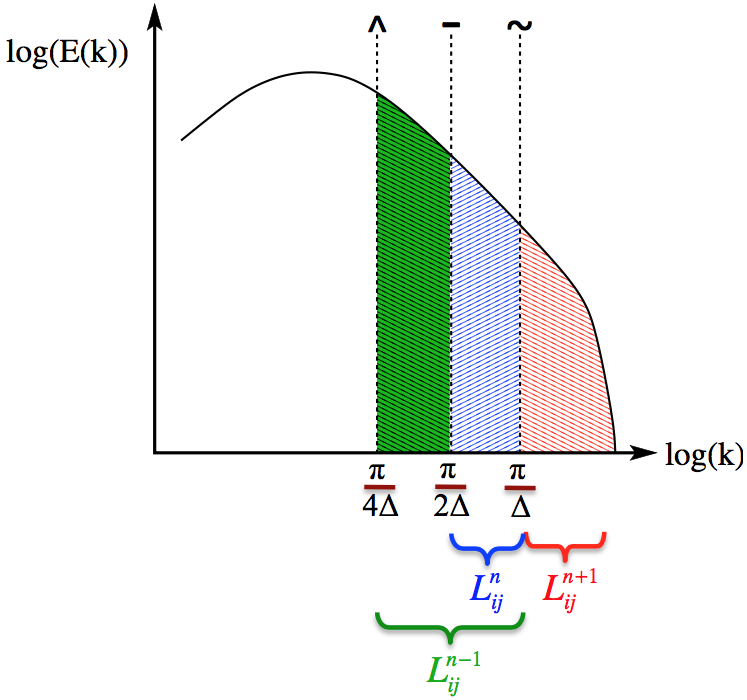
\includegraphics[width=0.6\textwidth]{scalesimilarity}
	\end{figure}

\end{itemize}
\end{frame}

%------------------------------------------------

\begin{frame}{Similarity Models}
\begin{columns}[T]
    \begin{column}{.55\textwidth}
    \begin{minipage}[c][.6\textheight][c]{\linewidth}
    \begin{itemize}
	\item They concluded that because of this the Leonard stress $(\tau_{ij}^{n-1})$ is the best estimate
	$$\boxed{\tau_{ij} = C_L L_{ij}}$$
	where $L_{ij} = \left(\overline{\widetilde{u}_i\widetilde{u}_j} - \overline{\widetilde{u}_i}\; \overline{\widetilde{u}_j}\right)$ and $C_L\sim 1$ is a dimensionless coefficient
	\item This is the most commonly used form (currently) of the similarity model
\end{itemize}
      \end{minipage}
    \end{column}
    \begin{column}{.55\textwidth}
      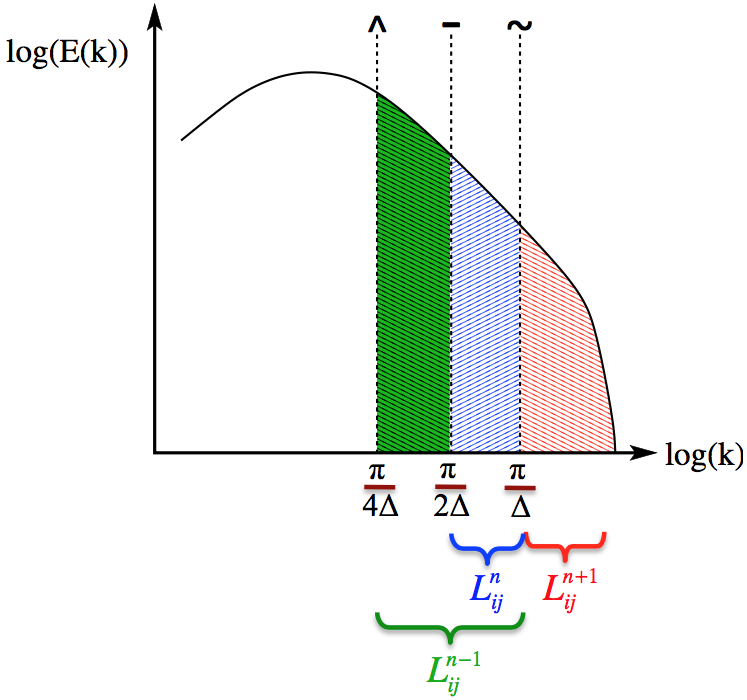
\includegraphics[width=\textwidth]{scalesimilarity}
    \end{column}
  \end{columns}
 \end{frame}
  
%------------------------------------------------

\begin{frame}{Similarity Models}
\begin{itemize}
	\item The Bardina and Liu models lead to high correlations between $\tau_{ij}^{\Delta}(\vec{x},t)$ and $\tau_{ij}^{\Delta,M}(\vec{x},t)$
	\item However, these models are expensive computationally due to the application of multiple explicit filtering operations
	\item Another procedure was introduced that reduces this cost, called the nonlinear model (a.k.a. Clark model, gradient model, or tensor-diffusivity model)
\end{itemize}

\end{frame}

%------------------------------------------------

\begin{frame}{Similarity Models}
\begin{itemize}
	\item The idea behind the nonlinear model is to approximate $\widetilde{u}_i$ by a Taylor series expansion around the ``true'' mean at a point
	$$\widetilde{u}_i(\vec{x}) = \overline{\widetilde{u}_i} + \widetilde{A}_{ijk}(\vec{x_0})(x_k - x_k^0)$$
	where $\widetilde{A}_{ijk}$ is the filtered gradient tensor, given by
	$$\widetilde{A}_{ijk}=\frac{\partial \widetilde{u}_i}{\partial x_k}$$
\end{itemize}

\end{frame}

%------------------------------------------------

\begin{frame}{Similarity Models}
\begin{itemize}
	\item We can use this approximation (Taylor series) to estimate the ``resolved'' stress $L_{ij} = \overline{\widetilde{u}_i \widetilde{u}_j} - \overline{\widetilde{u}_i}\;\overline{\widetilde{u}_j}$ (more later during discussion of dynamic modeling) and develop another model
	$$\boxed{\tau_{ij} = C_A \Delta^2 \widetilde{A}_{ik}\widetilde{A}_{jk}}$$
	\item Here we have used the observation that $\tau_{ij}$ has a very high correlation with $L_{ij}$
	$$\Rightarrow \tau_{ij} = C_A L_{ij}$$
	\item See Sagaut pg 231-231 for an example derivation
\end{itemize}

\end{frame}

%------------------------------------------------

\begin{frame}{Similarity Models}
\begin{itemize}
	\item The model shares the same order of deviation from the actual $\tau_{ij}$ as the Bardina-type models
	\item The primary advantage is that no additional explicit filtering operations are required
	\item As a result, the model is far less computationally expensive
\end{itemize}

\end{frame}

%------------------------------------------------



\end{document}

